\subsection{Ausgangssituation}
In der heutigen Zeit nimmt die Technik einen großen Einfluss auf unser Leben.
Jeder durchschnittliche Haushalt besitzt mindestens einen Computer mit
Internetanschluss und die meisten Leute haben heutzutage auch ein Smartphone.
Selten allerdings bleibt es bei diesen beiden Gerätschaften und so kommt zum Beispiel
ein Notebook für die Schule oder für den Arbeitsplatz zum Einsatz. Oftmals
müssen dabei die selben Dateien auf verschiedenen Geräten bearbeitet werden und
das möglichst ohne \glspl{versionconflict}. Daten müssen von jedem
Gerät und zu jederzeit erreichbar sein, weshalb Cloud- und
Dateisynchronisationsdienste einen immer größer werdenden Stellenwert bekommen.
Das Verwalten beziehungsweise die Verarbeitung von Daten in einer
zentrale Stelle, meistens einem Server und die dahinter liegende Datenbank des
jeweiligen Anbieters, soll dabei mit hoher Uptime den dauerhaften Zugriff auf
die eigenen Dateien sicherstellen.

\subsection{Funktionsweise üblicher Dateisynchronisationsdienste}
Die Idee hinter \sblit basiert auf den sicherheitsbezogenen Problemen, die mit
der Speicherung von Daten auf einer zentralen Stelle einhergehen. Die
Erleuterung der Funktionsweise üblicher Dateisynchronsationsdienste soll beim
Verstehen der grundsätzlichen Idee hinter \sblit helfen.

% TODO  Bild "Dropbox_1" einfügen
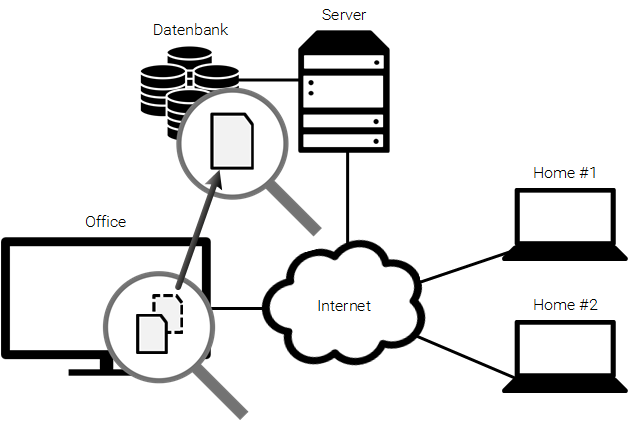
\includegraphics[]{images/Dropbox_1}
Üblich gehandhabtes Uploaden einer Datei.

Bei der Synchronisation einer Datei von einem Heimrechner zu einem Laptop am
Arbeitsplatz oder in der Schule wird eine Kopie dieser Datei auf den vom
Betreiber zur Verfügung gestellten Cloadspeicher beziehungsweise Server
hochgeladen und dort gespeichert. Der Sender behält dabei die Originaldatei.

% TODO  Bild "Dropbox_2" einfügen
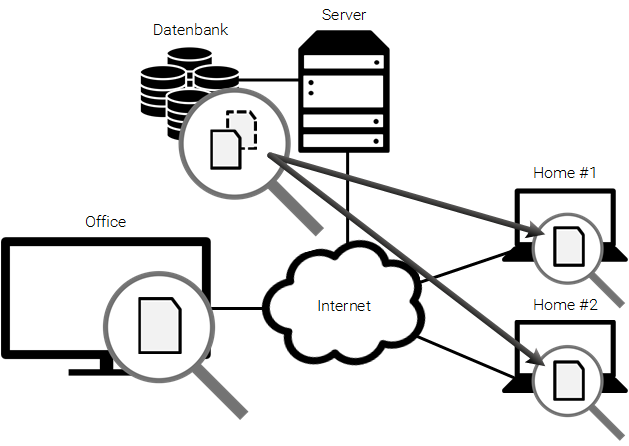
\includegraphics[]{images/Dropbox_2}
Üblich gehandhabtes Downloaden einer Datei.

Wenn der Laptop (TODO) in diesem Beispiel verfügbar ist, wird er über die Änderung
im Cloadspeicher informiert und lädt die Änderung, in diesem Fall die Datei von
dem Server herunter. Die Datei wurde somit über eine zentrale Stelle, hier den
Server synchronisiert.

\subsection{Problematik}
Ereignisse wie "The Fappening" oder diverse Hackerangriffe auf große Firmen, bei
denen Unmengen an Kundendaten gestohlen werden, zeigen wie leicht Mengen an
privaten Daten in falsche Hände fallen können, wenn diese zentral an einem Ort
gespeichert werden.

Geheimdienste oder staatliche Sicherheitsbehörden haben außerdem ein leichtes
Spiel an Userdaten heranzukommen, wenn sie gesammelt auf den Servern eines
Unternehmens gespeichert werden. Diese Unternehmen sind als Anbieter solcher
Cloudspeicher unter Umständen zur Herausgabe der Nutzerdaten gesetzlich
verpflichtet.

Und selbst wenn der duchschnittliche Benutzer nichts zu verbergen hat, ist der
dreiste Eingriff in die Privatsphäre doch als äußerst problematisch einzustufen
und leider gestaltet sich dieser zum Bedauern der betroffenen Benutzer, für
Fremden oft viel zu einfach.

\subsection{Idee}
Hauptursache für diese Problematik ist die oft unverschlüsselte, zentrale
Speicherung der Daten. Damit aber nicht auf den Komfort verzichtet werden muss,
der von üblichen Dateisynchronisationsdiensten geboten wird, werden die zuvor angesprochenen
Probleme bei \sblit umgangen.

Bei \sblit werden Dateien anstatt über einen Server, nämlich über verschlüsselte
\glspl{p2plink} zwischen zwei Endgeräten direkt übertragen.
Oft kommt es allerdings vor, dass \glspl{syncpartner} beim Verändern von
Dateien nicht erreichbar sind und kein \gls{p2plink} aufgebaut und auch
keine Datei synchronisiert werden kann.
Mit dem Senden einer neuen Version von Dateien zu warten,
bis beide Clients gleichzeitig erreichbar sind, hätte eine zu große Zeitspanne
zur Folge, in der viele Versionskonflikte auftreten könnten.
Deshalb verwendet \sblit eine Cloud, um Dateien für nicht erreichbare
Synchronisationspartner extern zwischenspeichern zu können. Die Cloud bildet
sich dabei aber nicht aus einem Server, wie üblich, sondern aus einem \gls{p2pnet}
aller Nutzer von \sblit. Diese dezentrale \gls{Filecloud} wird
mit sogenannten \gls{partnership} realisiert. Dabei geht es darum, dass sich
User, die sich gegenseitig nicht kennen müssen, einander ihre Daten direkt über
verschlüsselte Kanäle auf den Geräten des jeweiligen anderen speichern.
Um die Dateien nicht nur sicher zu übertragen, sondern auch zwischenzuspeichern
ohne, dass Dritte Zugriff haben, werden die zu
synchronisierenden Dateien in Blöcke aufgeteilt und verschlüsselt. Diese
verschlüsselten Blöcke werden dann verteilt auf die Partnergeräte gespeichert,
sodass diese fremden User nichts damit anfangen können, da sie weder den
Schlüssel zum Entschlüsseln, noch die Informationen über den Ort der restlichen
Blöcke besitzen. Diese befindet sich ausnahmslos nur bei dem User, zu dem die
Blöcke gehören.

\subsubsection{Szenario}
Bei \sblit wird der Inhalt eines Ordners synchronisert, der bei der
Konfiguration angegebenen wurde. Sobald sich Dateien innerhalb des Ordners
ändern, wird die neue Version der Datei kopiert und die Kopie wird den
erreichbaren Synchronisationspartnern über einen \gls{p2plink}
gesendet.

% TODO Bild "sblit_1" einfügen
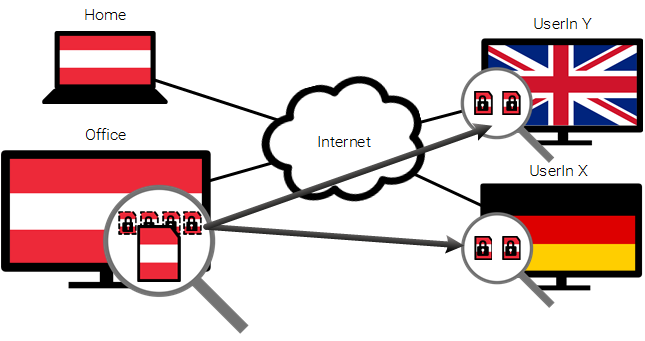
\includegraphics[]{images/sblit_1}
Übertragung der Datei zwischen zwei erreichbaren Hosts.

Für Synchronisationspartner, die nicht erreichbar sind, wird die Datei in der
\gls{dezentralen Filecloud} zwischengespeichert. Die Datei wird kopiert und in Blöcke
aufgeteilt. Diese Blöcke werden mit dem privaten Schlüssel des Clients
verschlüsselt und verteilt auf den \glspl{partnerdevice} gespeichert.

Da die Erreichbarkeit der Partnergeräte, auf denen die veschlüsselten
Datei-Blöcke gespeichert sind, nicht gewährleistet ist, wird die Datei mehrmals
in die \gls{dezentrale Filecloud} gespeichert, sodass nur ein Bruchteil der
Partnergeräte erreichbar sein muss, um auf die vollständige Datei zugreifen zu
können.

% TODO Bild "sblit_2" einfügen
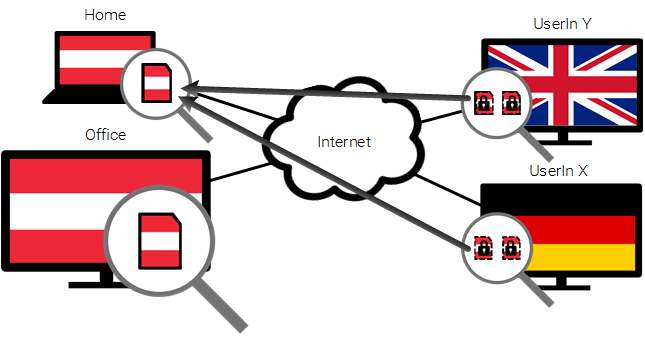
\includegraphics[]{images/sblit_2}
Hochladen der Datei in die dezentrale Filecloud.

Sobald der Synchronisationspartner, hier Home_1 wieder erreichbar, also dem
\gls{p2pnet} beigetreten ist, fordert er die verschlüsselten
Dateiblöcke von den \glspl{partnerdevice} an. Verschlüsselte \glspl{p2plink}
werden aufgebaut und die Blöcke werden übertragen, entschlüsselt und zu der
vollständigen Datei zusammengesetzt.

Die Datei wurde also über die Partnergeräte synchronisiert, die eine dezentrale
Filecloud darstellen.

% TODO Bild "sblit_3"
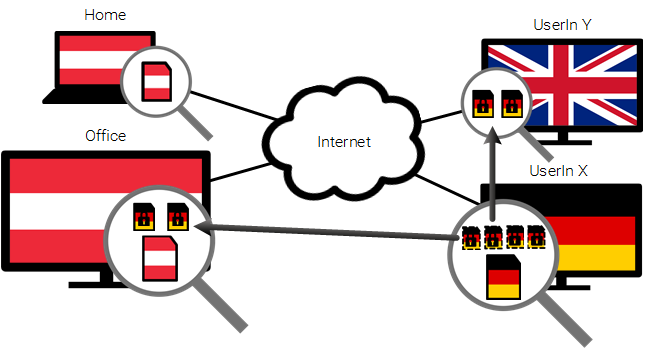
\includegraphics[]{images/sblit_3}
Gegenseitiges Speichern von Dateiblöcken (Konzept einer \gls{partnership}).

Im Gegenzug, dass man Daten auf Geräten anderer speichern darf, gibt man selbst
Speicherplatz für diese User frei, in dem die von ihnen verschlüsselten
Dateiblöcke zwischengespeichert werden können. Der für andere User freigegebene
Speicherplatz beträgt dabei die Speichermenge, die man selbst bei anderen Usern
beansprucht.
